Consider the execution depicted in Figure~\ref{fig:read}~(a), where state variables $x$ is created on partition $\ppm_1$ in the middle of the execution of S-SMR. Command $C_1(x)$ and $C_3(x)$ reads the value of $x$, $C_2(x,\ppm_1)$ create $x$ on partition $\ppm_1$. Client a first multicasts query to the $Oracle$ for location of $x$, which is not available at that time, hence $Oracle$ return empty result, which tell client a to end the execution. Client b then wants to create variable $x$ on $\ppm_1$, before sending actual creating command, client b also multicasts query to $Oracle$ to get the involved partition (eg., $\ppm_1$), then multicasts $C_2(x,\ppm_1)$ to both $Oracle$ and $\ppm_1$. Oracle will update information of $x$, and $\ppm_1$ will execute create $x$ command. From then, for every read command to $x$ (eg., $C_3(x)$), $Oracle$ could answer with partition $\ppm_1$ which is the one holds $x$.

\begin{figure*}
\begin{minipage}[b]{1.0\linewidth} % A minipage that covers the whole width of the page
\centering
      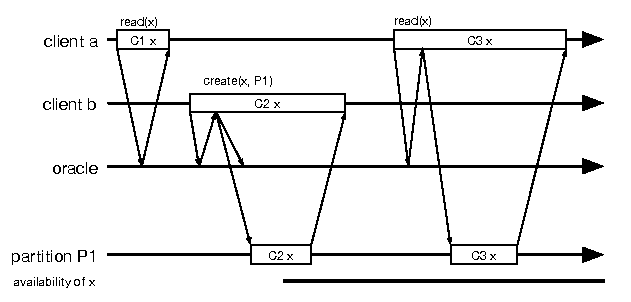
\includegraphics[width=0.6\linewidth]{figures/read_simple}
\end{minipage}
\centering
	\caption{Execution flow of DS-SMR with $create$ command}
\label{fig:read}
\end{figure*}

In the following figures~(\ref{fig:readoverlap}b, \ref{fig:readoverlap}c), where read command $C_1(x)$ comes in the middle of the execution of create command $C_2(x,\ppm_1)$, while the query of $C_1(x)$ comes after multicasts command of $C_2(x,\ppm_1)$. With the knowledge of $x$, Oracle response to the query with a positive answer, therefore there are possibilities that the read command either comes during (eg., fig.~\ref{fig:readoverlap}b) or before (eg., fig.~\ref{fig:readoverlap}c) the execution of actual write command. The SSMR model avoid the problem described in figure~\ref{fig:readoverlap}~(b) by ensuring that the execution of every command is atomic (eg., for every server $s$ in partition $\ppm$ that executes $C$, there is a server $r$ in every $\ppm' \in part(C)$ such that $delivery(C,r) < end(C,s)$. Intuitively, this condition guarantees that the execution of $C_1$ and $C_2$ at $\ppm$ overlap in time). Atomic multicast prevents the problem figure~\ref{fig:readoverlap}~(c) from happening as $deliver(C_2) \prec deliver(C_1)$, that leads to situation described in fig.~\ref{fig:readoverlap}b.

\begin{figure*}
\begin{minipage}[b]{1.0\linewidth} % A minipage that covers the whole width of the page
\centering
      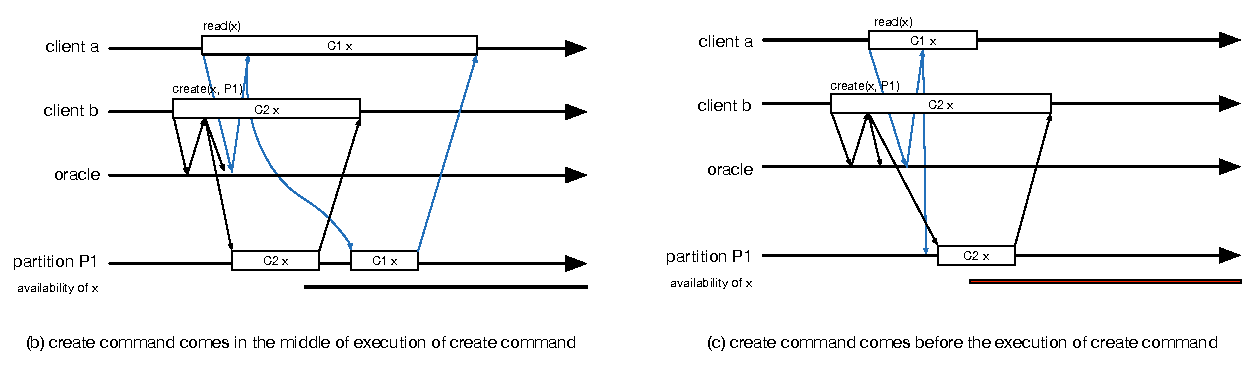
\includegraphics[width=1\linewidth]{figures/read_overlap}
\end{minipage}
\caption{Execution flow of D-SSMR with overlapping read-create commands}
\label{fig:readoverlap}
\end{figure*}


Next figure~(\ref{fig:updateoverlap} a, \ref{fig:updateoverlap} b) depicts the scenario of moving object location from a partition to another. Intuitively, the problem with the execution in fig.~\ref{fig:updateoverlap}a is that read command $C_3(x)$ executes “in between” the execution of $C_2(x,\ppm_2)$ at partitions Px and Py. Before sending $C_3$ to destination partition, client 1 send query to oracle for possible position of $x$, which is $P_1$ at that specific moment, but not correct at the execution time. In D-SSMR, we prevent that from happening by using oracle as the controller for accessing state variable on partitions, by using versioning mechanism on oracle for different type of commands. Whenever a client sends a command that update variable $C(x)$, oracle also increases the version of that variable $x$ in its knowledge. 
% Then after the associated process execute command $C$, it also tell Oracle to release the lock $L$, and inform the oracle about the update of $x$ (if there is any).

There are possibilities that a client could fail in the middle of the execution of the command chains, at the moment after requires the lock and before sending the actual $C$ command to partition $P$. In this case, TODO: which one release lock, either oracle or another client that require lock again. 

\begin{figure*}
\begin{minipage}[b]{1.0\linewidth} % A minipage that covers the whole width of the page
\centering
      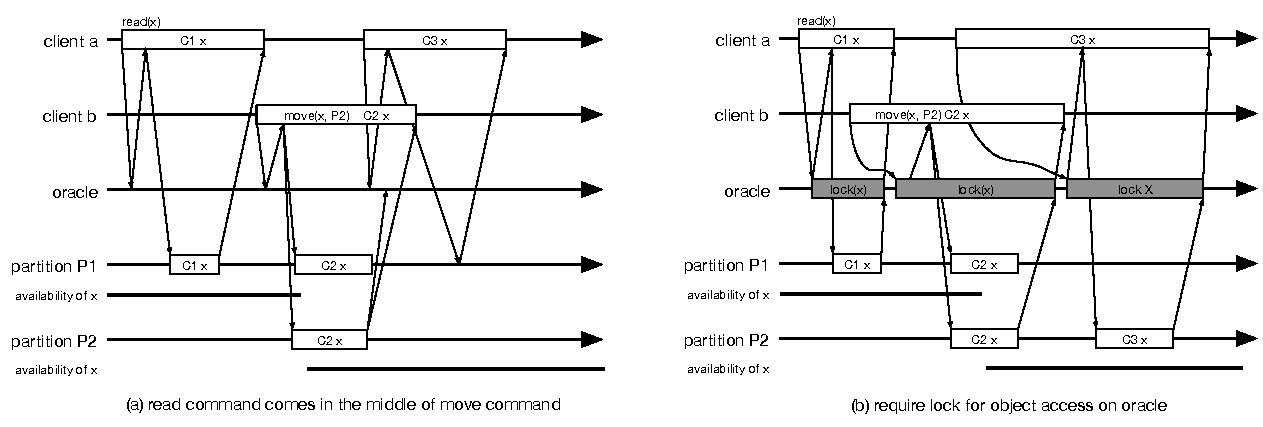
\includegraphics[width=1\linewidth]{figures/update_overlap}
\end{minipage}
\caption{Execution flow of DS-SMR with overlapping read-update commands}
\label{fig:updateoverlap}
\end{figure*}


\subsection{Detailed algorithm}
\label{sec:detailalg}

In Algorithm \ref{alg:dssmr}, we show the operation of DS-SMR. 
To submit a command $C$, the client first check its cache to get the lastest information $dests$ of the state objects in command. Then it can either uses that info if exists, or sends a query to the Oracle to get set $dests$~(line \ref{algline:query_oracle}, \ref{algline:oracle_response}), which is a superset of $part(C)$ used by the client as destination set for $C$~(line \ref{algline:cli_mcast}). 

Upon delivering $Q(C)$, oracle $O$ runs function $getPart(C)$ which returns a set $\vvm$ of involved state variables of command $C$. If there exists a variable $v_i \in \vvm$ in oracle memory, which indicates the variable $v_i$ exists on a partition $p_i \in \ppm$, oracle reply to client with $p_i$ value, or an empty result otherwise. In addition, upon delivering $C(v, \ppm)$, oracle update its memory with new location of $v$: $\vvm\_part\{v.id\} \leftarrow \ppm$

If the $dests$ from Oracle is empty, client stop the command there. (line \ref{algline:cli_terminate})

Upon delivering $C$, server $P$ execute $C$ and reply to the client. 
% Upon delivering $C$, server $s$ in partition \pp\ multicasts $signal(C)$ to $others$, which is the set containing all other partitions involved in $C$ (lines \ref{algline:others} and \ref{algline:mcastsignals}). 
% %The purpose of $signal(C)$ is to let servers in other partitions know that there is a server in \pp\ that started executing $C$. 
% It might happen that $s$ receives signals concerning $C$ from other partitions even before $s$ started executing $C$. For this reason, $s$ must buffer signals and check if there are signals buffered already when starting the execution of $C$. For the sake of simplicity, Algorithm \ref{alg:ssmr} simply initializes such buffers as $\emptyset$ for all possible commands. In practice, buffers for $C$ are created when the first message concerning $C$ is delivered.

% After multicasting signals, server $s$ proceeds to the execution of $C$, which is a sequence of operations that might read or write variables in \vv. The main concern is with operations that read variables, as they may determine the outcome of the command execution. All other operations can be executed locally at $s$. If the operation reads variable $v$ and $v$ belongs to \pp, $s$'s partition, then $s$ multicasts the value of $v$ to the other partitions that delivered $C$ (line \ref{algline:multicastv}). The command identifier $C.id$ is sent along with $v$ to make sure that the other partitions will use the appropriate value of $v$ during $C$'s execution. If $v$ belongs to some other partition $\ppm'$, $s$ waits until an up-to-date value of $v$ has been delivered (line \ref{algline:waitvariable}). Every other operation is executed with no interaction with other partitions (line \ref{algline:executeopck}).

% After executing all operations of $C$, $s$ waits until a signal from every other partition has been received (line \ref{algline:waitsignals}) and, only then, sends the reply back to the client (line \ref{algline:sendreply}). This ensures that $C$ will be execution atomic.



% Upon delivering $C$, server $s$ in partition \pp\ multicasts $signal(C)$ to $others$, which is the set containing all other partitions involved in $C$ (lines \ref{algline:others} and \ref{algline:mcastsignals}). 
% %The purpose of $signal(C)$ is to let servers in other partitions know that there is a server in \pp\ that started executing $C$. 
% It might happen that $s$ receives signals concerning $C$ from other partitions even before $s$ started executing $C$. For this reason, $s$ must buffer signals and check if there are signals buffered already when starting the execution of $C$. For the sake of simplicity, Algorithm \ref{alg:dssmr} simply initializes such buffers as $\emptyset$ for all possible commands. In practice, buffers for $C$ are created when the first message concerning $C$ is delivered.